\chapter{Appendix}


\section{On the influence of several factors on pathway enrichment analysis}
\label{ap:review}

\vspace*{1cm}

\noindent
Reprinted with permission from "Mubeen S., Kodamullil A.T., Hofmann-Apitius M., and Domingo-Fern\'{a}ndez D. (2022). On the influence of several factors on pathway enrichment analysis  \textit{Briefings in Bioinformatics}, 23(3)".

\noindent
Copyright © Mubeen, S., \textit{et al.}, 2022.

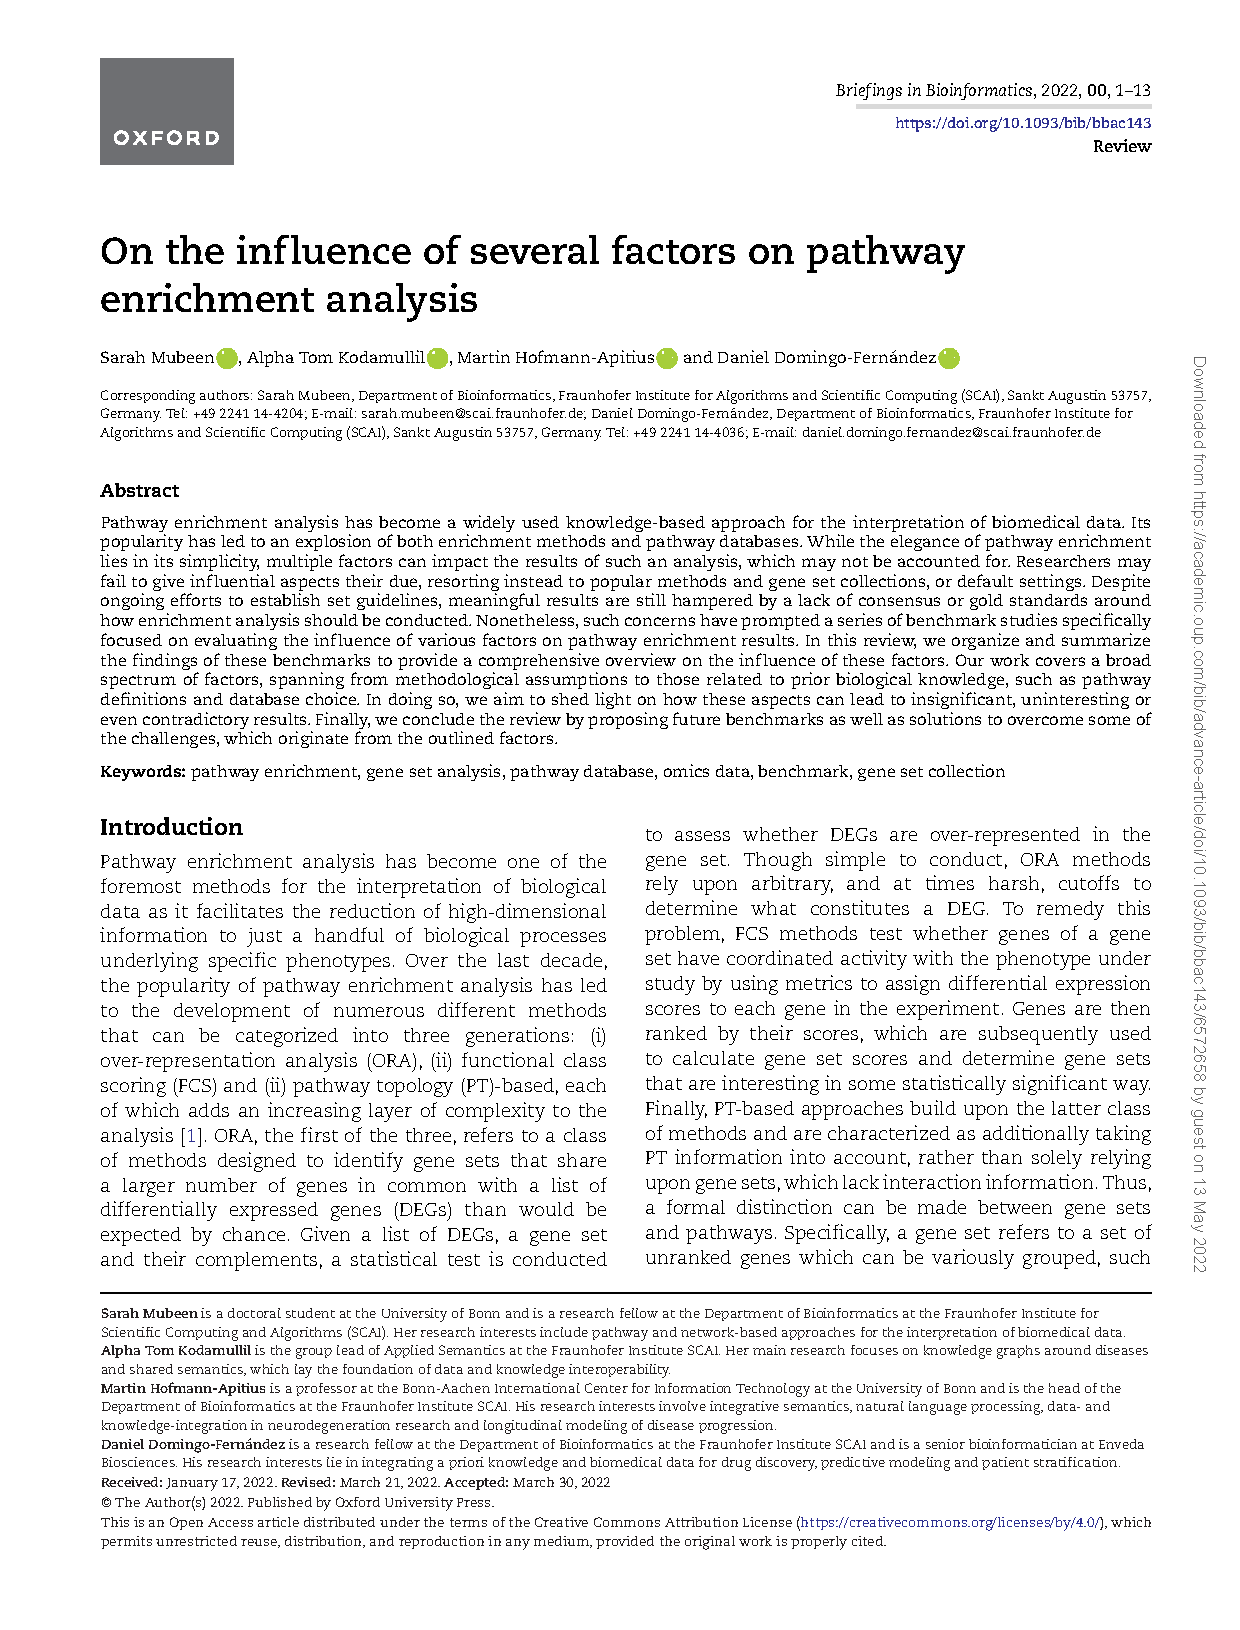
\includepdf[pages={-}]{doctoral_thesis/articles/review.pdf}



\section{The Impact of Pathway Database Choice on Statistical Enrichment Analysis and Predictive Modeling}
\label{ap:pathwayforte}

\vspace*{2cm}

\noindent
Reprinted with permission from "Mubeen S., Hoyt C. T., Gemünd A., Hofmann-Apitius M., Fröhlich H., and Domingo-Fern\'{a}ndez D. (2019). The Impact of Pathway Database Choice on Statistical Enrichment Analysis and Predictive Modeling. \textit{Frontiers in Genetics}, 10:1203".

\noindent
Copyright © Mubeen, S., \textit{et al.}, 2019

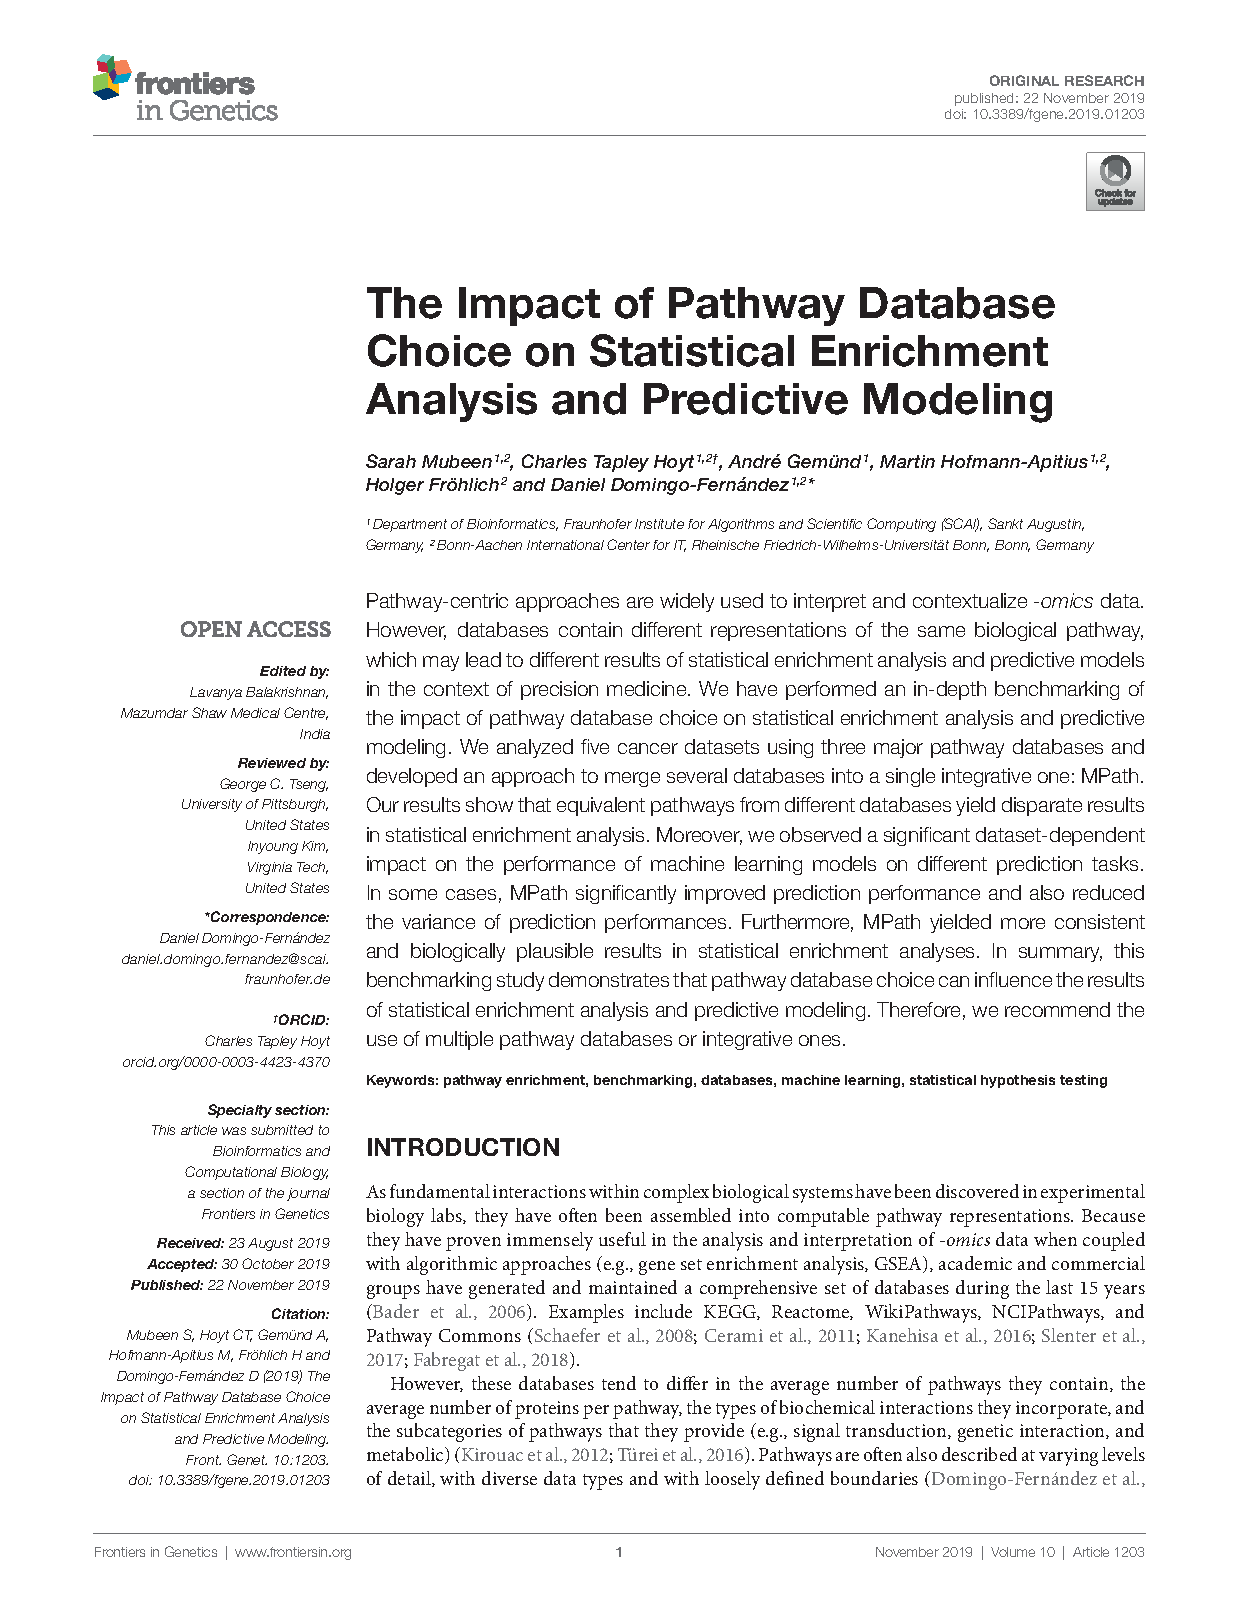
\includepdf[pages={-}]{doctoral_thesis/articles/pathwayforte.pdf}



\section{DecoPath: a web application for decoding pathway enrichment analysis}
\label{ap:decopath}

\vspace*{2cm}

\noindent
Reprinted with permission from "Mubeen S., Bharadhwaj S. V., Kodamullil A.T., Gadiya Y., Hofmann-Apitius M., and Domingo-Fern\'{a}ndez D. (2021). DecoPath: A Web Application for Decoding Pathway Enrichment Analysis.  \textit{NAR Genomics and Bioinformatics}, 3(3): lqab087".

\noindent
Copyright © Mubeen, S., \textit{et al.}, 2021.

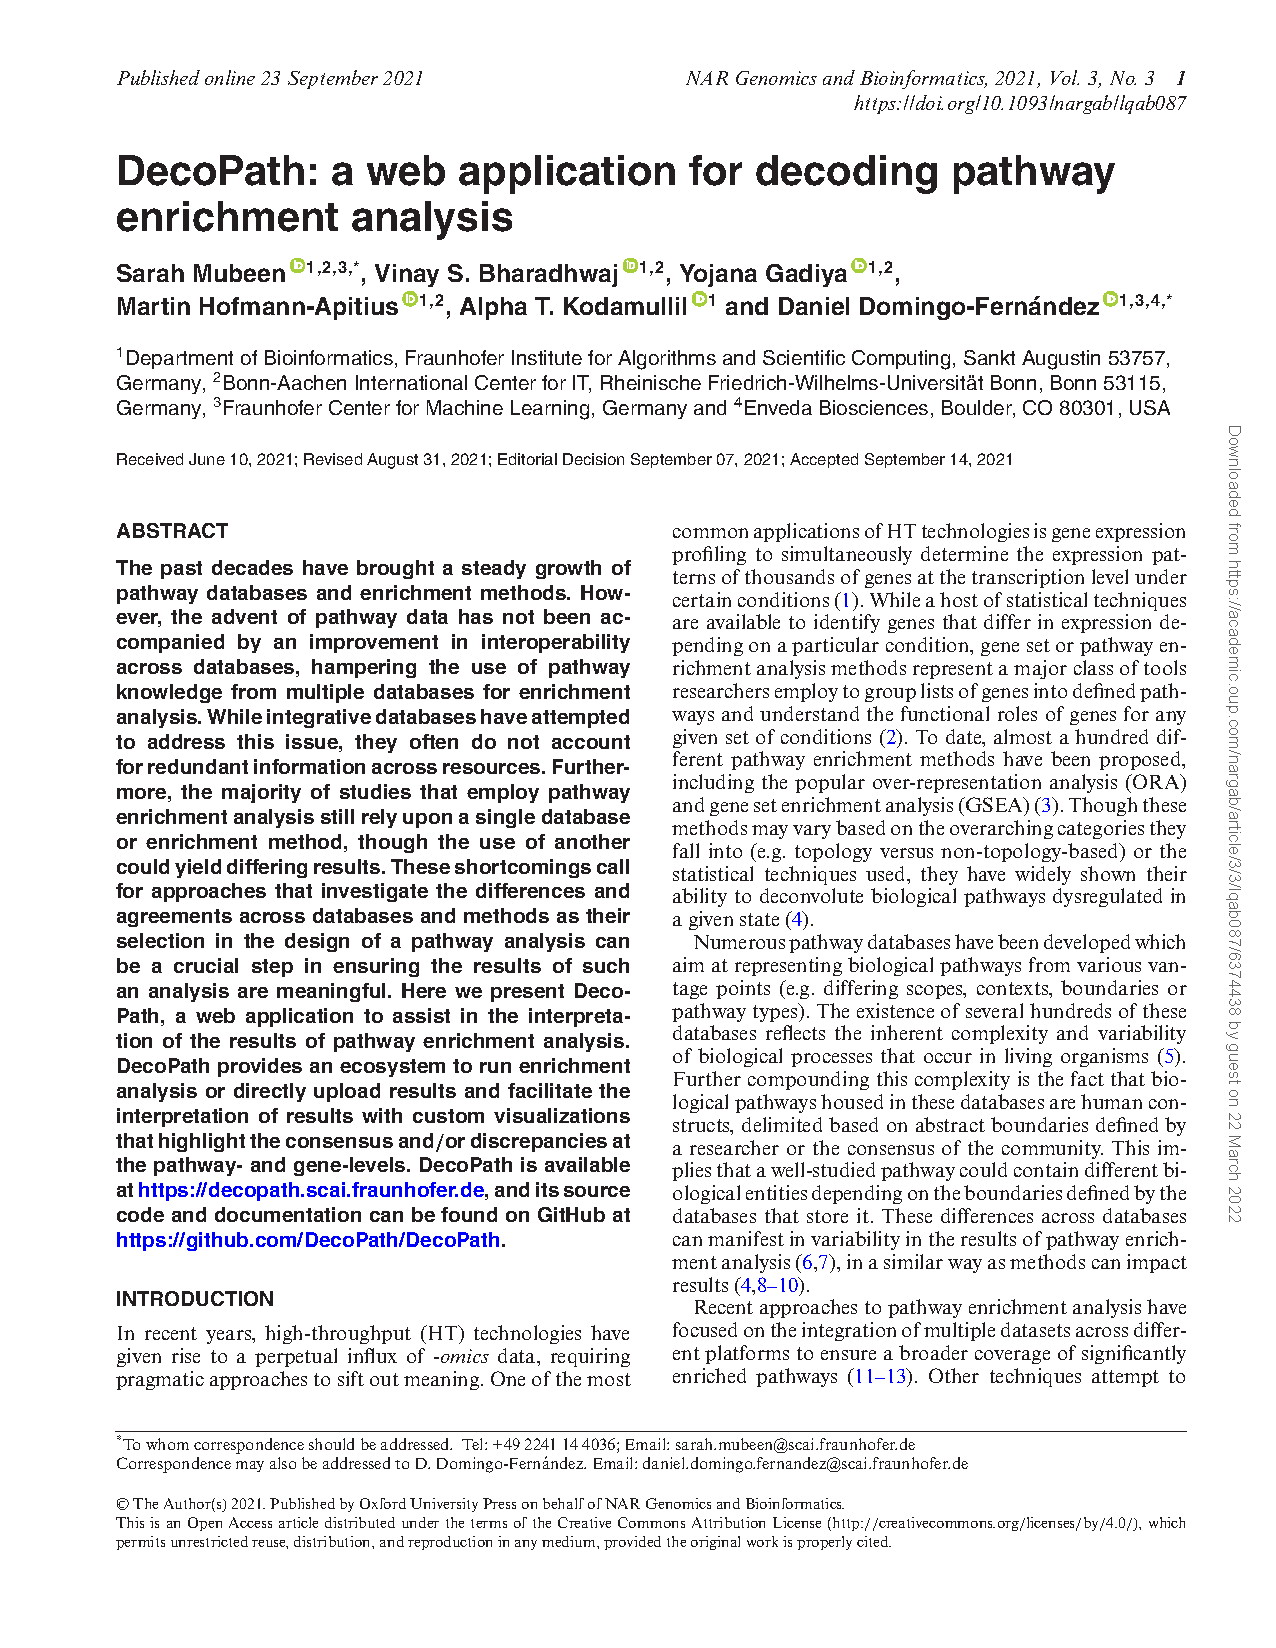
\includepdf[pages={-}]{doctoral_thesis/articles/decopath.pdf}



\section{Towards a global investigation of transcriptomic signatures through co-expression networks and pathway knowledge for the identification of disease mechanisms}
\label{ap:coxpath}

\vspace*{2cm}

\noindent
Reprinted with permission from "Figueiredo R.Q., Raschka T., Kodamullil AT., Hofmann-Apitius M., Mubeen S.\textsuperscript{\textdagger}, and Domingo-Fern\'{a}ndez D.\textsuperscript{\textdagger} (2021). Towards a global investigation of transcriptomic signatures through co-expression networks and pathway knowledge for the identification of disease mechanisms. \textit{Nucleic acid research}, 49(14): 7939–7953".

\noindent
Copyright © Figueiredo R.Q., \textit{et al.}, 2021.

\includepdf[pages={-}]{doctoral_thesis/articles/coxpath.pdf}



\section{Elucidating gene expression patterns across multiple biological contexts through a large-scale investigation of transcriptomic datasets}
\label{ap:contnext}

\vspace*{2cm}

\noindent
Reprinted with permission from "Figueiredo R.Q., Díaz del Ser S., Raschka T., Hofmann-Apitius M., Kodamullil A.T., Mubeen S.\textsuperscript{\textdagger}, and Domingo-Fern\'{a}ndez D.\textsuperscript{\textdagger} (2022). Elucidating gene expression patterns across multiple biological contexts through a large-scale investigation of transcriptomic datasets. \textit{BMC Bioinformatics}, 23(1)".

\noindent
Copyright © Figueiredo R.Q., \textit{et al.}, 2022.

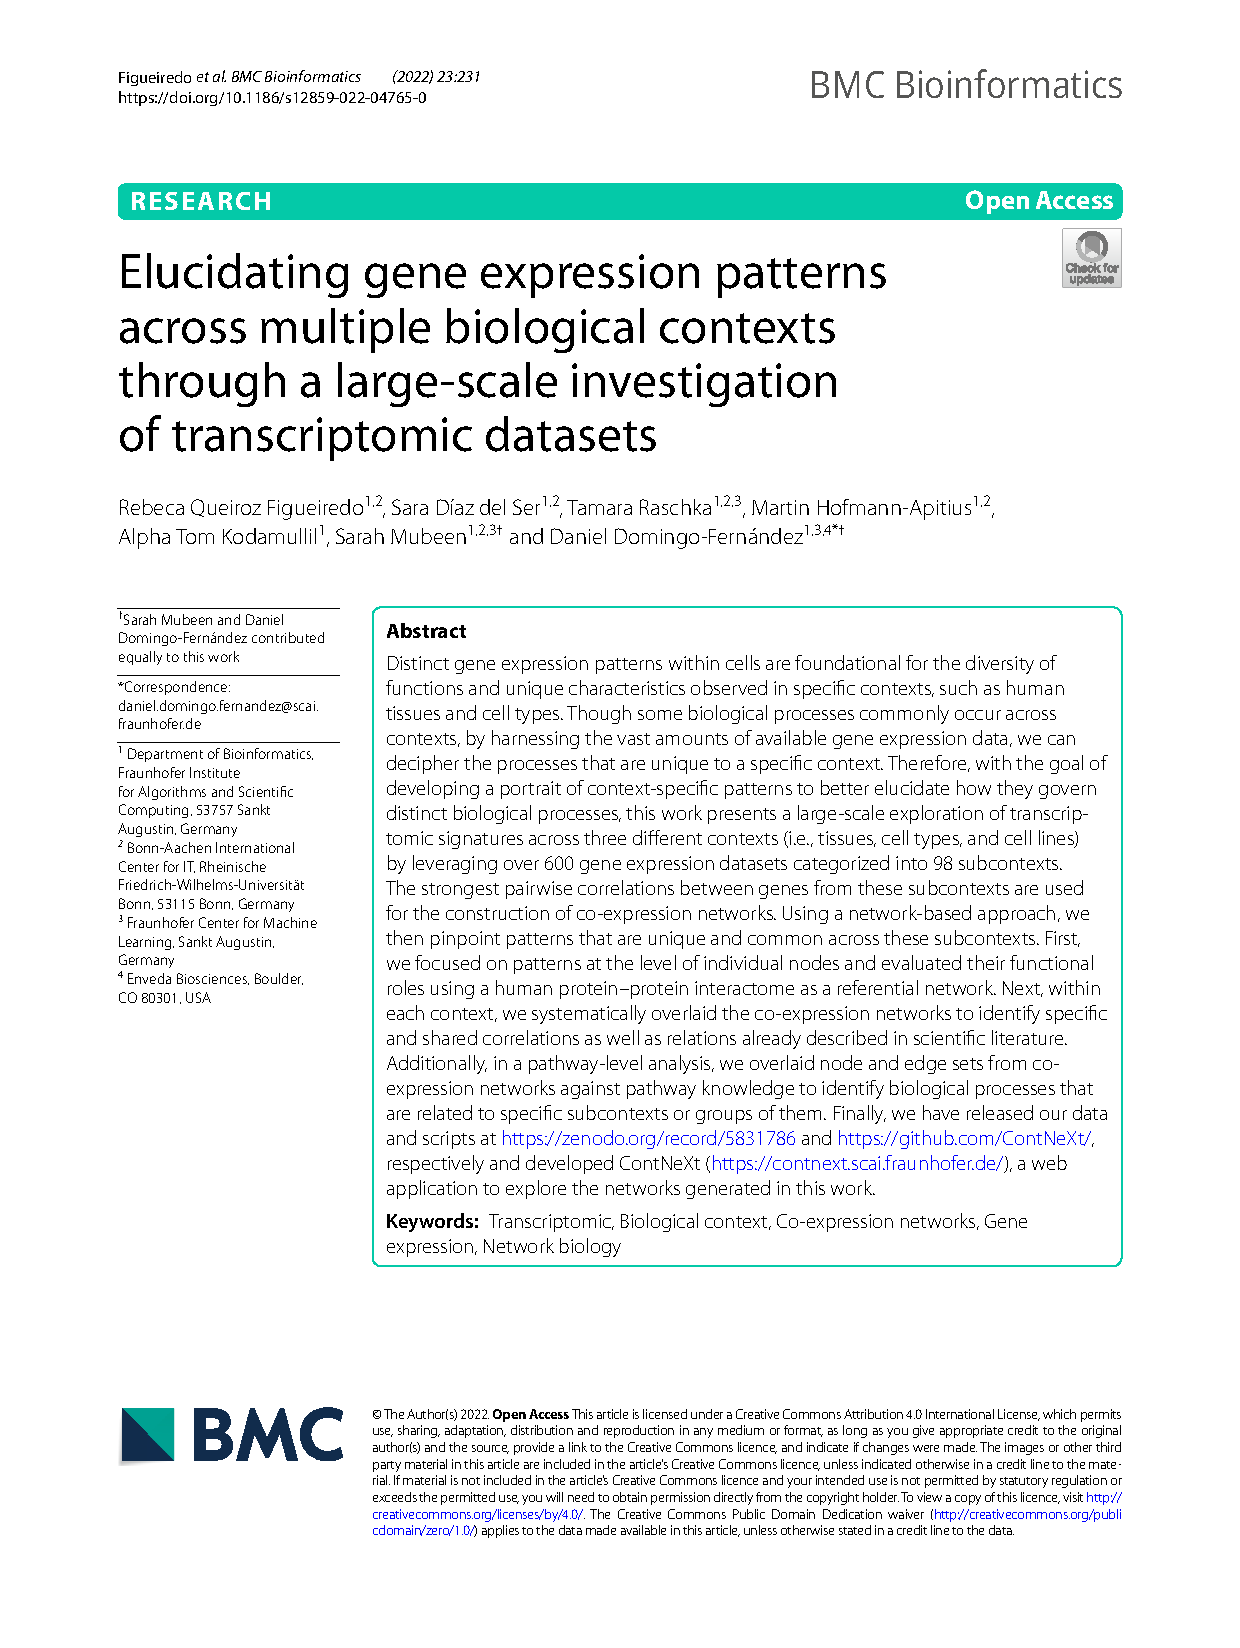
\includepdf[pages={-}]{doctoral_thesis/articles/contnext.pdf}
 


\section{MultiPaths: a Python framework for analyzing multi-layer biological networks using diffusion algorithms}
\label{ap:multipaths}

\vspace*{2cm}

\noindent
Reprinted with permission from "Marín-Llaó J., Mubeen S., Perera-Lluna A., Hofmann-Apitius M., Picart-Armada S., and Domingo-Fern\'{a}ndez D. (2021). MultiPaths: a Python framework for analyzing multi-layer biological networks using diffusion algorithms. \textit{Bioinformatics}, 37(1): 137-139".

\noindent
Copyright © Marín-Llaó, J., \textit{et al.}, 2021.

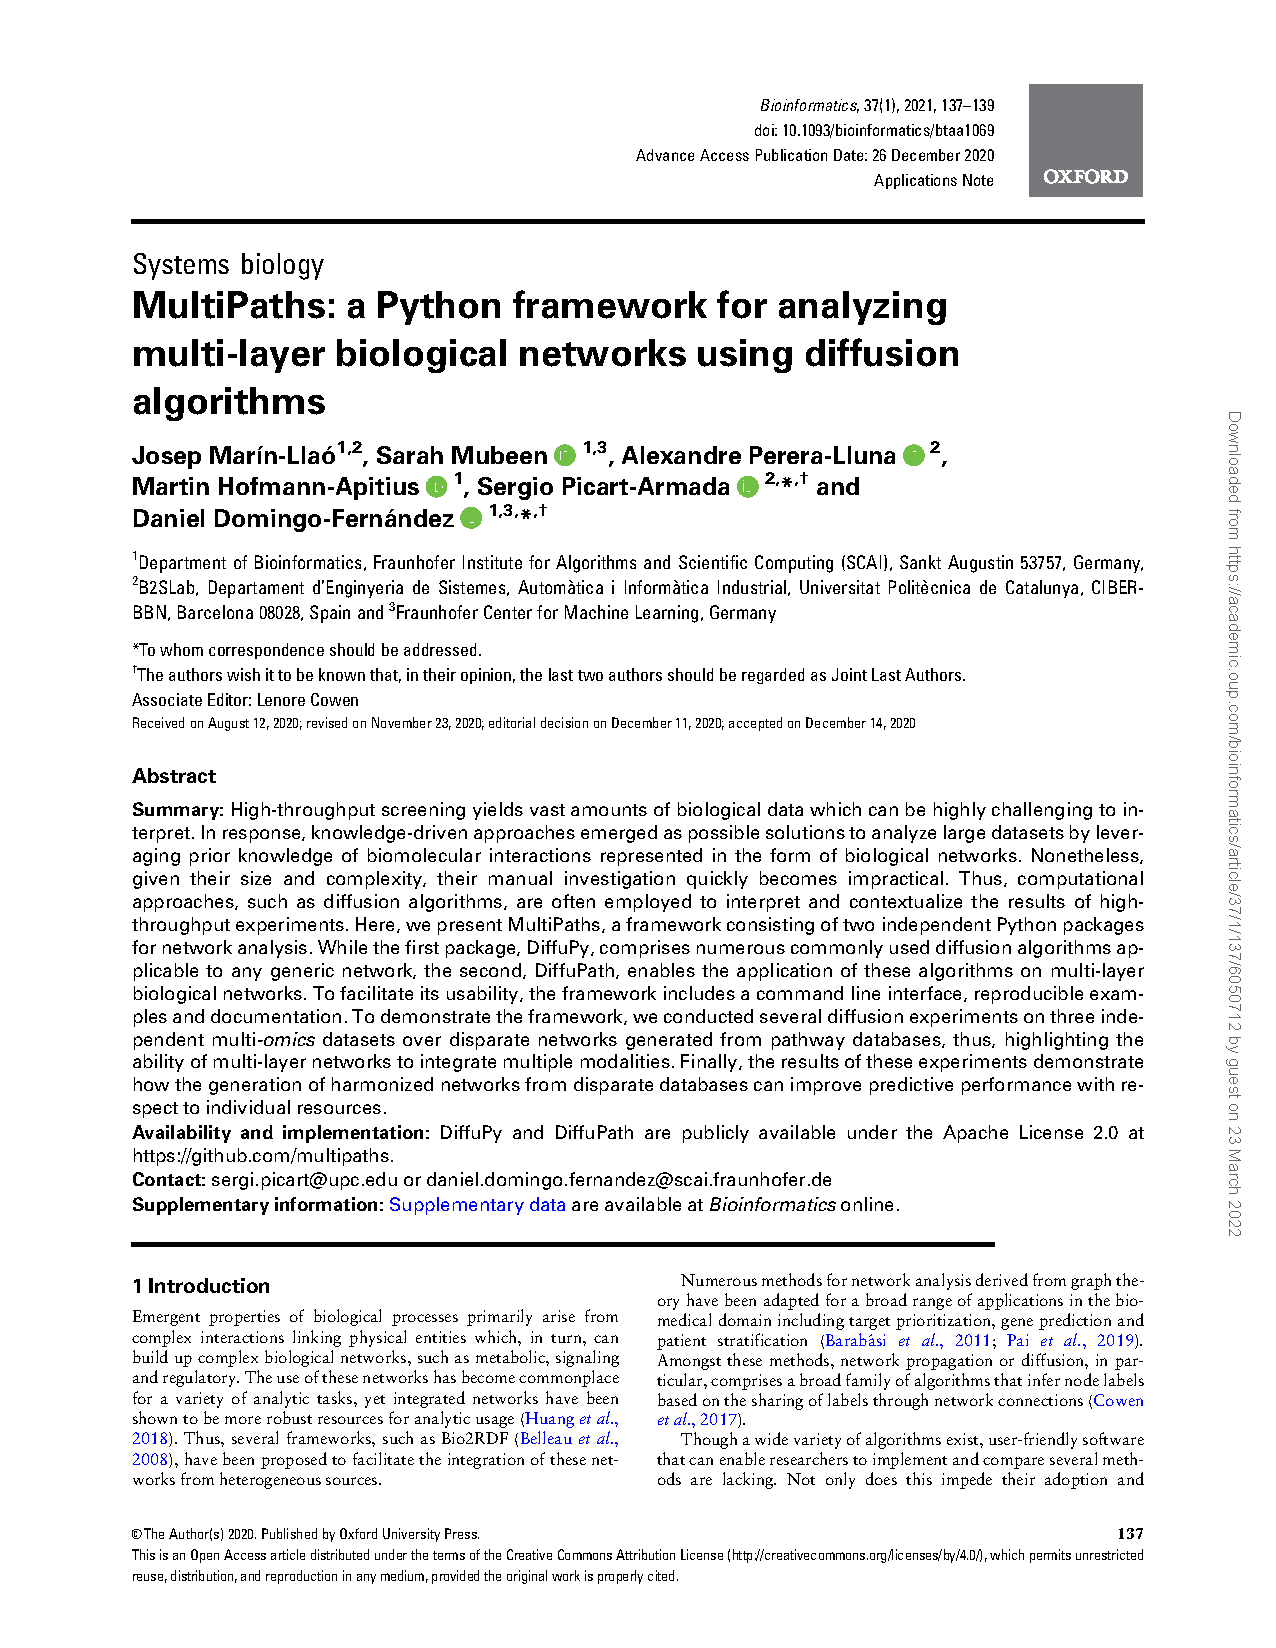
\includepdf[pages={-}]{doctoral_thesis/articles/multipaths.pdf}



\section{Drug2ways: reasoning over causal paths in biological networks for drug discovery}
\label{ap:drug2ways}

\vspace*{2cm}

\noindent
Reprinted with permission from "Rivas-Barragan D., Mubeen S., Guim Bernat F., Hofmann-Apitius M., and Domingo-Fern\'{a}ndez D. (2020). Drug2ways: Reasoning over causal paths in biological networks for drug discovery. \textit{PLOS Computational Biology}, 16(12): e1008464".

\noindent
Copyright © Rivas-Barragan D., \textit{et al.}, 2020.

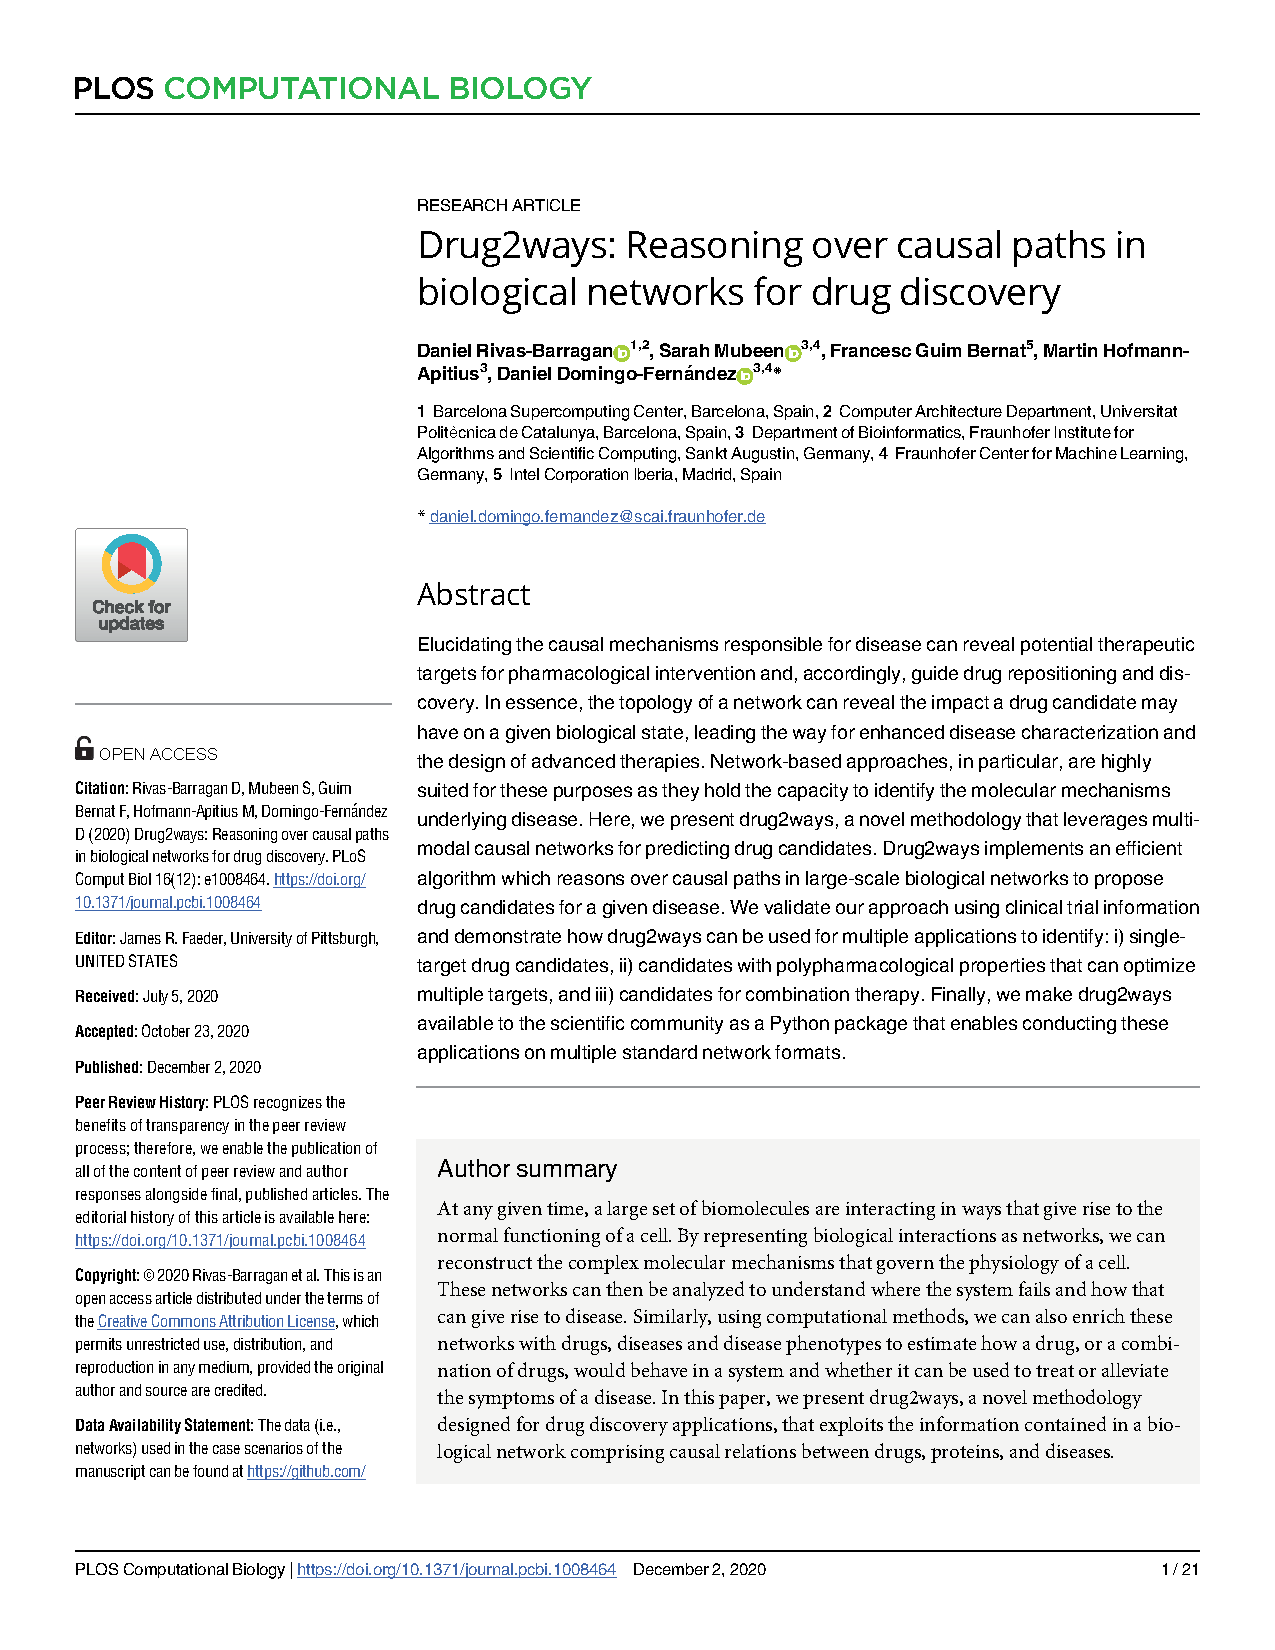
\includepdf[pages={-}]{doctoral_thesis/articles/drug2ways.pdf}
